\documentclass{article}
\usepackage{iclr2026_conference,times}

\input{math_commands.tex}

\usepackage{hyperref}
\usepackage{url}
\usepackage{graphicx}

% Extra math for this paper
\usepackage{amsthm}
\theoremstyle{plain}
\newtheorem{theorem}{Theorem}[section]
\theoremstyle{definition}
\newtheorem{definition}[theorem]{Definition}
\newtheorem{remark}[theorem]{Remark}
\newcommand{\ip}[1]{\langle #1 \rangle}

\title{Low-Rank Networks Learn High-Frequency Features}

% Authors must not appear in the submitted version.
\author{Anonymous Author(s)
}

%\iclrfinalcopy
\begin{document}

\maketitle

\begin{abstract}
We study how low-rank random feature (RF-LR) and matrix-rank (MMNN) networks learn representations through \emph{channel feature learning}: in our setting, different low-rank channels specialize to distinct spatial locations and progressively capture higher-frequency components. We combine a tractable mean-field toy model with a rigorous \emph{log-ratio criterion} that characterizes when one channel dominates at a given input location, and we validate the predictions with controlled experiments. We then report an \emph{empirical study of oscillatory complexity across layers}: for MMNNs trained on 1D regression, we define the mean number of strictly-positive local minima per component of the layer-wise partial functions and show that this statistic increases with layer index, consistent with deeper layers learning more oscillatory representations. The pipeline is reproducible; scope is limited to the RF-LR/MMNN setting and 1D regression. Results align with the SciForDL focus on empirical studies of learned representations and training dynamics.
\end{abstract}

\section{Introduction}
\label{sec:intro}

Understanding how deep networks learn representations remains a central challenge. The Science of Deep Learning workshop promotes controlled experiments and tractable models to test precise hypotheses. In that spirit, we focus on \emph{feature learning} in low-rank neural networks (RF-LR with frozen random features, and MMNNs): how the $r$ low-rank channels organize representations across space and frequency.

Low-rank architectures factorize weights and reduce parameters while preserving expressivity. In our setting, different channels specialize: each channel tends to dominate near a \emph{distinct spatial value} (localization), and channels separate by \emph{frequency} (lower first, then higher). We summarize the feature-learning and \emph{log-ratio} analysis from the mean-field treatment of RF-LR networks, then present a \emph{controlled empirical study} of oscillatory complexity in MMNNs using the number of strict local minima per partial-function component as a proxy for how oscillatory a layer's representation is. \textbf{Scope:} the theory applies to the RF-LR toy setting; the oscillatory-complexity results are for 1D regression and the reported architecture; we do not claim generalization beyond this setting without further experiments.

\section{Setup: RF-LR and channel partial functions}
\label{sec:setup}

We consider a low-rank random feature network. The first layer uses frozen random features $L^0(C_1)$; the second layer has a frozen mixing matrix $L$ of rank $r$ and trainable weights $w_1(t,C_1,k)$, $w_2(t,C_2)$. The second-layer pre-activation is $H_2(t,c_2;X,W) = \sum_{k=1}^r L_{c_2,k}\,f_k(t;X,W)$, where the \emph{channel partial functions} are $f_k(t;X,W) = \E_{C_1}[w_1(t,C_1,k)\,\varphi_1(\ip{L^0(C_1)}{X})]$. The backpropagated signal is $B_k(t;X,W) = \E_{C_2}[L_{C_2,k}\,\varphi_2'(H_2(t,C_2;X,W))\,w_2(t,C_2)]$. The kernel induced by the frozen first layer is $K_{\mu_0}(x,x')$ (NNGP-type). The mean-field evolution for $f_k$ is
\begin{equation}
\label{eq:fk-evol}
\partial_t f_k(t,x) = -\xi_1(t)\,\E_{Z=(X,Y)}[d_L(Z;W(t))\,B_k(t;X)\,K_{\mu_0}(x,X)].
\end{equation}

\section{Mechanism of spike learning}
\label{sec:mechanism}

When channel $k$ dominates at $x_0$, $H_2 \approx L_{c_2,k}f_k$ there, so $\varphi_2'(H_2)$ is effectively driven by that channel. The backprop signal $B_k$ aggregates over the second layer; once a channel dominates, the dynamics create \emph{emergent} sign-coherence and a self-reinforcing loop: larger dominance $\to$ larger $B_k$ $\to$ larger $\partial_t f_k$ $\to$ further amplified dominance. The log-ratio criterion (Theorem~\ref{thm:logratio}) formalizes that \emph{when} certain conditions hold on an interval $I$, dominance cannot be lost on $I$.

\section{Two-sided step toy model and log-ratio criterion}
\label{sec:toy}

Consider the \emph{two-sided step}: two support points $x_0=-\delta$, $x_1=+\delta$ with $y(x_0)=+A$, $y(x_1)=-A$. For this finitely supported data, $f_k$ takes the form $f_k(t,x) = f_k(0,x) - \Gamma_{k,1}(t)\,K_{\mu_0}(x,x_0) - \Gamma_{k,2}(t)\,K_{\mu_0}(x,x_1)$, with $\Gamma_{k,p}(t) = \int_0^t \xi_1(s)\,d_p(s)\,B_{k,p}(s)\,ds$. The full evolution at $x_p$ is $\partial_t f_k(t,x_p) = -\xi_1(t)\,K_{\mu_0}(x_p,x_p)\,d_p(t)\,B_{k,p}(t) + E_p(t)$, with $|E_p(t)|\le C'\,\psi(\delta)$, $\psi(\delta)\to 0$ as $\delta\to\infty$.

\begin{definition}[Log-ratio criterion]
At $x_0$, define $R_{12}(t,x_0) = \log\frac{|f_1(t,x_0)|}{|f_2(t,x_0)|}$.
\end{definition}

\begin{theorem}[Log-ratio growth at $x_0$ (conditional)]
\label{thm:logratio}
\textbf{Setting:} Two-sided step, $r=2$ channels, 3-layer RF-LR.

\textbf{Hypothesis (at $x_0$, for all $t\in I$):} (i) $-d_0(t)\ge 0$; (ii) $B_{1,1}(t)$ has the same sign as $f_1(t,x_0)$; (iii) $|B_{2,1}(t)|\le \rho_0\,\frac{|f_2(t,x_0)|}{|f_1(t,x_0)|}\,|B_{1,1}(t)|$ for some $\rho_0\in[0,1)$.

\textbf{Conclusion:} For $t\in I$, $\partial_t R_{12}(t,x_0) = (1-\rho_0)\,\xi_1(t)\,K_{\mu_0}(x_0,x_0)\,(-d_0(t))\,\frac{|B_{1,1}(t)|}{|f_1(t,x_0)|} + \varepsilon_0(t)$, with $|\varepsilon_0(t)|\le C''\,\psi(\delta)$. Hence $\partial_t R_{12}(t,x_0)\ge 0$ whenever the leading term dominates $|\varepsilon_0|$. Strict dominance of channel 1 at $x_0$ cannot be lost on $I$. The result is symmetrical at $x_1$.
\end{theorem}

\begin{remark}
The theorem is conditional: it states that \emph{when} (i)--(iii) hold, the conclusion follows. In practice, (i)--(iii) are observed under standard initialization.
\end{remark}

\section{Experimental validation: log-ratio diagnostics}
\label{sec:experiments}

We validate the log-ratio on frequency-dependent function approximation. Setup: 3-layer low-rank ReLU, $n=1024$, $r=15$, target $f(x)=\cos(8\pi x)$ on $[-1,1]$, $N=5000$ samples. At $x=0$ we measure channel partials $f_k$ and log-ratios $R_{i,j}=\log|f_i|-\log|f_j|$. We observe that the trajectory of $\max_{i,j}R_{i,j}(x=0)$ shows sustained growth (one channel increasingly dominates), and the heatmap of $R_{i,j}$ over training exhibits the same specialization pattern. Newer log-ratio plots (over training and across locations) are more stable; a \textbf{uniform distribution in log space} of the ratios is a useful diagnostic for specialization---when channel dominance is well separated, the log-ratios spread and stabilize. A related phenomenon is \textbf{log-ratio collapse}: under some LR/batch regimes the log-ratios can collapse (e.g.\ all channels similar) or, conversely, diverge globally by end of training; scaling laws with batch size also appear (e.g.\ at lr $10^{-3}$, large batch 128 can perform very well in some configs). Figures~\ref{fig:logratio-div} and \ref{fig:logratio-conv} illustrate the contrast: at lr $2{\times}10^{-3}$, bs 4, trajectories diverge by end of training; at lr $2{\times}10^{-4}$, bs 4, they converge (stable specialization).

\begin{figure}[htbp]
\centering

\includegraphics[width=0.85\linewidth]{icml_sgdadamlandscapedynamical/figures/trajectory_max_ratio.png}
\caption{Trajectory of $\max_{i,j}R_{i,j}(x=0)$ vs.\ epoch. Setup: $n=1024$, $r=15$, $\cos(8\pi x)$.}
\label{fig:trajectory}
\end{figure}

\begin{figure}[htbp]
\centering
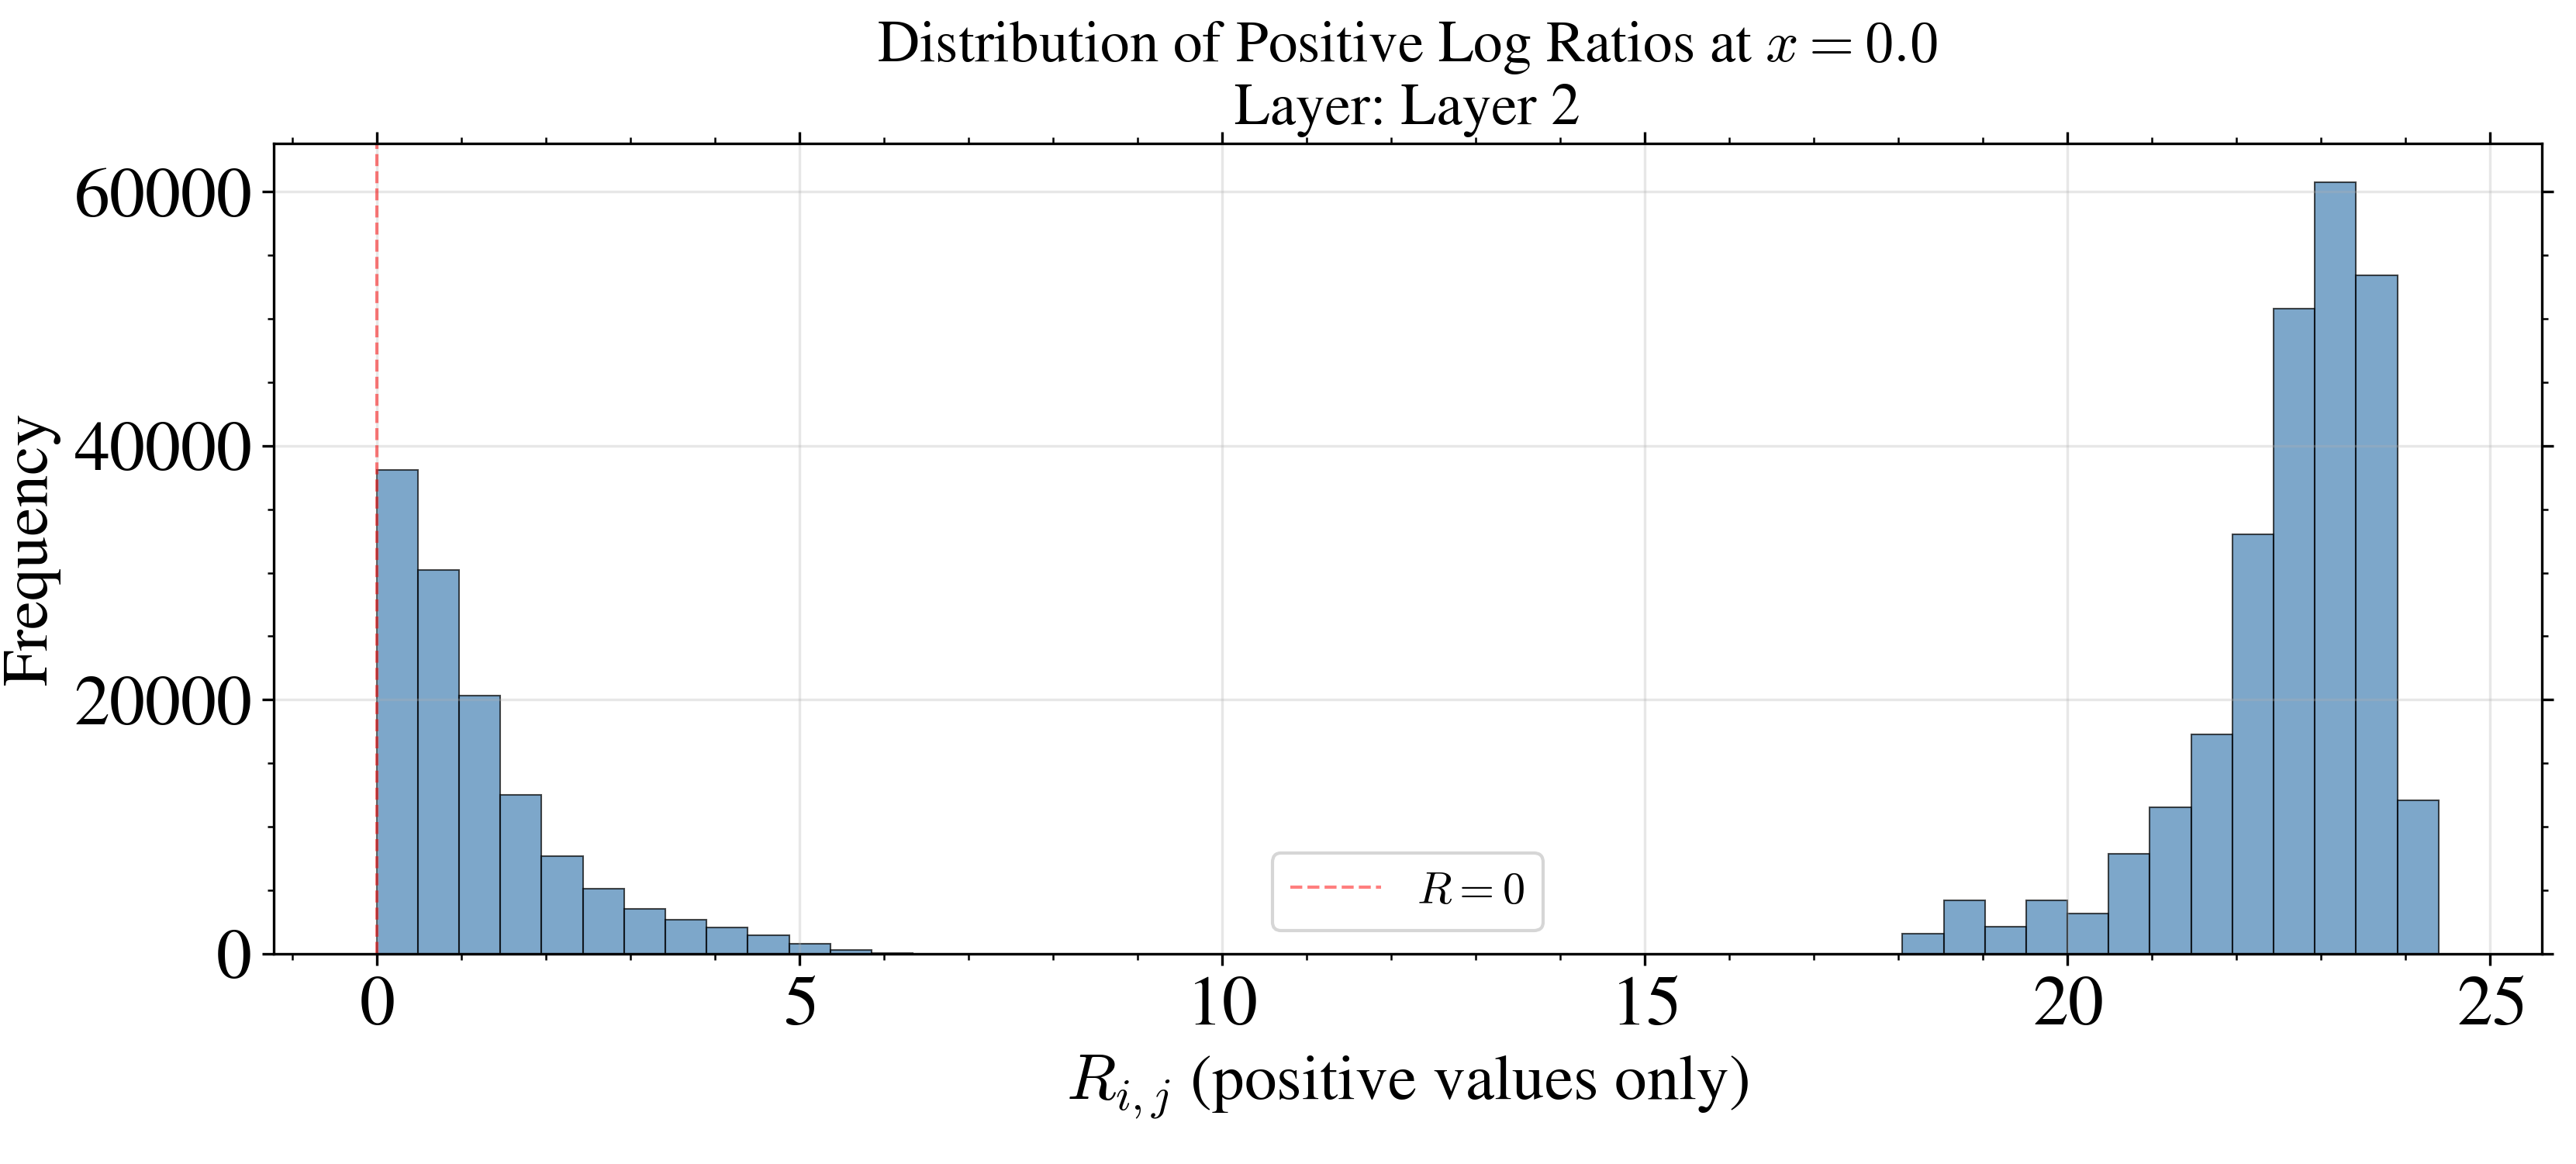
\includegraphics[width=0.85\linewidth]{icml_sgdadamlandscapedynamical/figures/logratio_statistics_x0.png}
\caption{Log-ratios $R_{i,j}$ at $x=0$ over training (all channel pairs).}
\label{fig:logratio-heatmap}
\end{figure}

\begin{figure}[htbp]
\centering
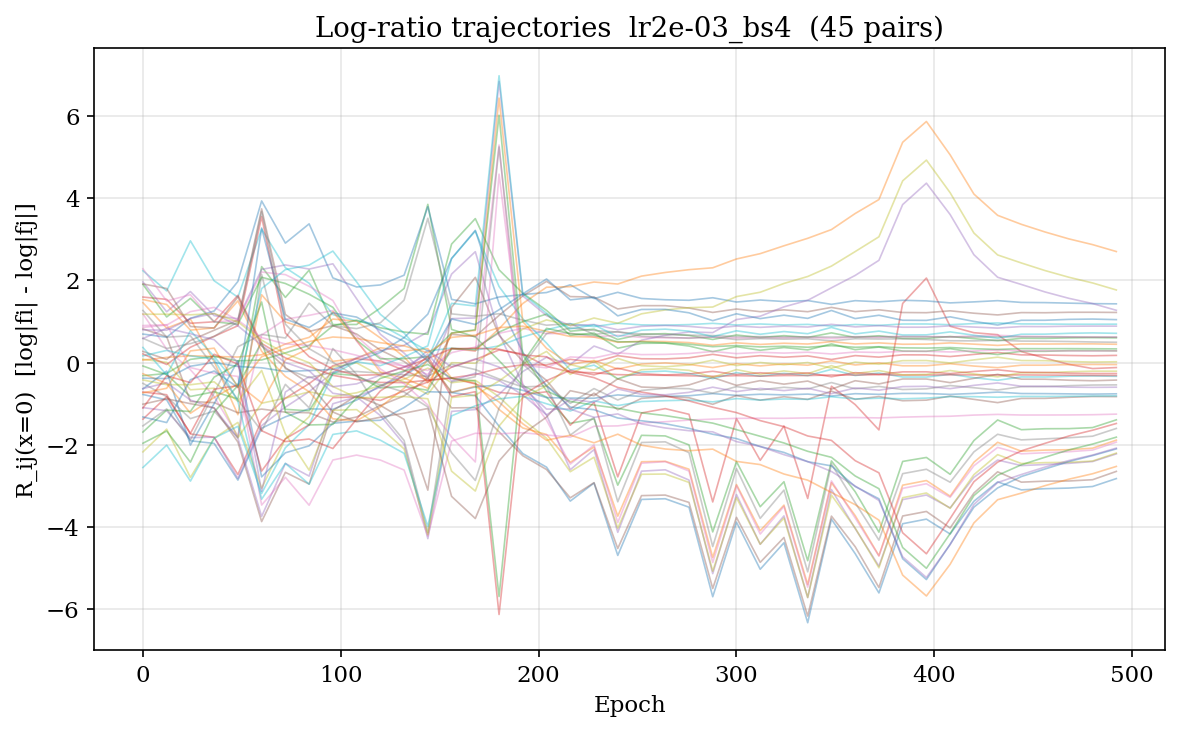
\includegraphics[width=0.85\linewidth]{figures/logratio_trajectories_lr2e-03_bs4_divergence.png}
\caption{Log-ratio trajectories; lr $2{\times}10^{-3}$, bs 4. Divergence by end of training.}
\label{fig:logratio-div}
\end{figure}

\begin{figure}[htbp]
\centering
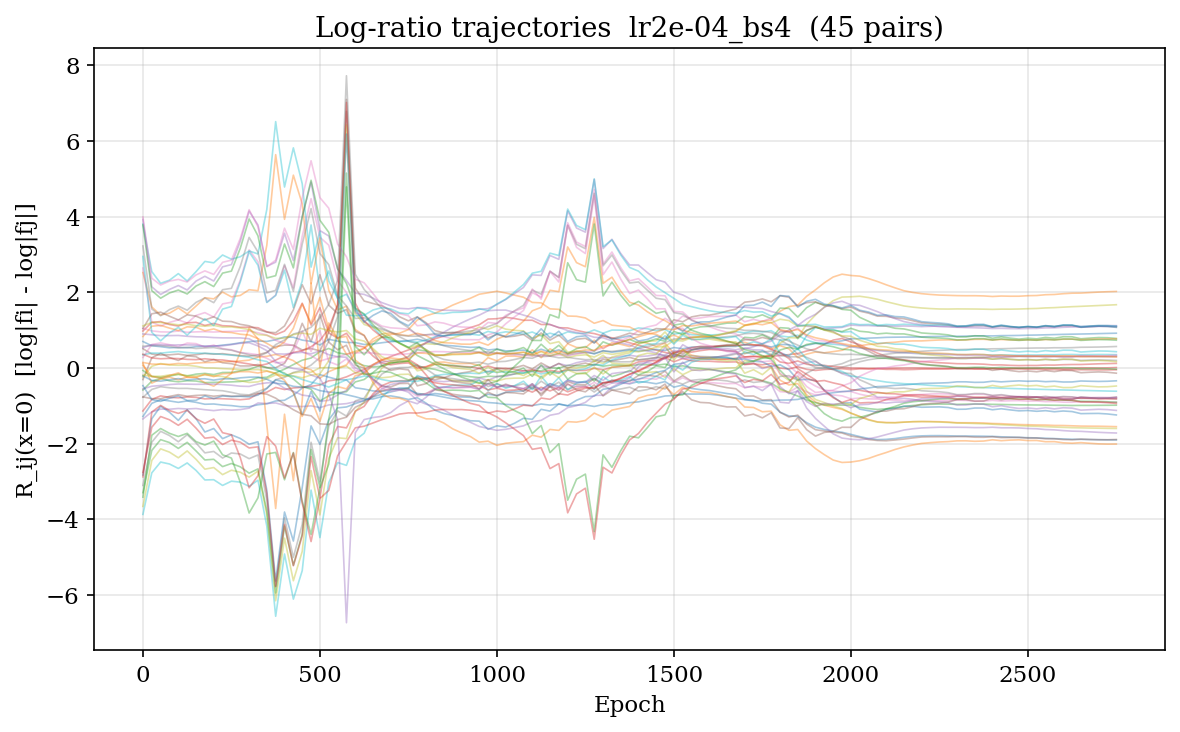
\includegraphics[width=0.85\linewidth]{figures/logratio_trajectories_lr2e-04_bs4_convergence.png}
\caption{Log-ratio trajectories; lr $2{\times}10^{-4}$, bs 4. Convergence (stable specialization).}
\label{fig:logratio-conv}
\end{figure}

\section{Empirical analysis of oscillatory complexity across layers}
\label{sec:oscillatory}

A natural hypothesis is that \emph{deeper layers} build increasingly complex, high-frequency internal representations. Testing this in a controlled way requires \emph{observable proxies} for ``oscillatory complexity'' computable from trained models. We focus on \textbf{matrix-rank neural networks (MMNNs)} trained on 1D regression. For each layer we have \textbf{partial functions} $h_\ell(x) \in \R^{d_\ell}$ (one scalar per channel) on $x \in [-1,1]$. A simple, interpretable proxy for how oscillatory a scalar function is along $x$ is the \textbf{number of strict local minima} above a positivity threshold $\varepsilon=10^{-4}$ (to ignore ReLU zero plateaus).

\subsection{Statistic and protocol}

For each component $h_{\ell,j}(x_i)$ on a uniform grid $x_1,\ldots,x_N$ ($N=1000$), we count a \emph{strict local minimum} at index $i$ if $h_{\ell,j}(x_i) < h_{\ell,j}(x_{i-1})$, $h_{\ell,j}(x_i) < h_{\ell,j}(x_{i+1})$, and $h_{\ell,j}(x_i) > \varepsilon$. The per-component count is $m_{\ell,j}$. The \textbf{layer-level statistic} is the mean number of minima per component:
\begin{equation}
\bar{m}_\ell = \frac{1}{d_\ell} \sum_{j=1}^{d_\ell} m_{\ell,j}.
\end{equation}
We also record boxplots and histograms across components. Models are trained on a 1D target (e.g.\ sum of cosines) with MSE; we use saved checkpoints and the same partial-function extraction as in the repository's leap analysis.

\subsection{Results}

In all runs we observe a \textbf{clear increase in $\bar{m}_\ell$ with layer index $\ell$} in the second half of the network. For $L=6$, $W=128$, and $R \in \{5,10,15,20,30,36,50\}$ (one run per $R$), early layers (1--4) have mean $\bar{m}_\ell \le 0.35$ for all groups; later layers (roughly 7--13) show mean counts from about 1 to 9, with the highest values at the last representation layer (e.g.\ layer 12: $\bar{m}_{12}$ ranges from 2.33 for $R=15$ to 8.60 for $R=5$; layer 14, scalar output, has a single count between 2 and 11 depending on $R$). Distributions across components are \textbf{right-skewed} and heterogeneous (e.g.\ at layer 12, quartiles differ strongly across $R$). This is consistent with the hypothesis that \textbf{deeper layers learn more oscillatory partial functions} under this discrete proxy. The dependence on rank $R$ is \textbf{not monotonic} in the current single-run-per-config data, so replication over seeds is needed to characterize rank effects.

\begin{figure}[htbp]
\centering
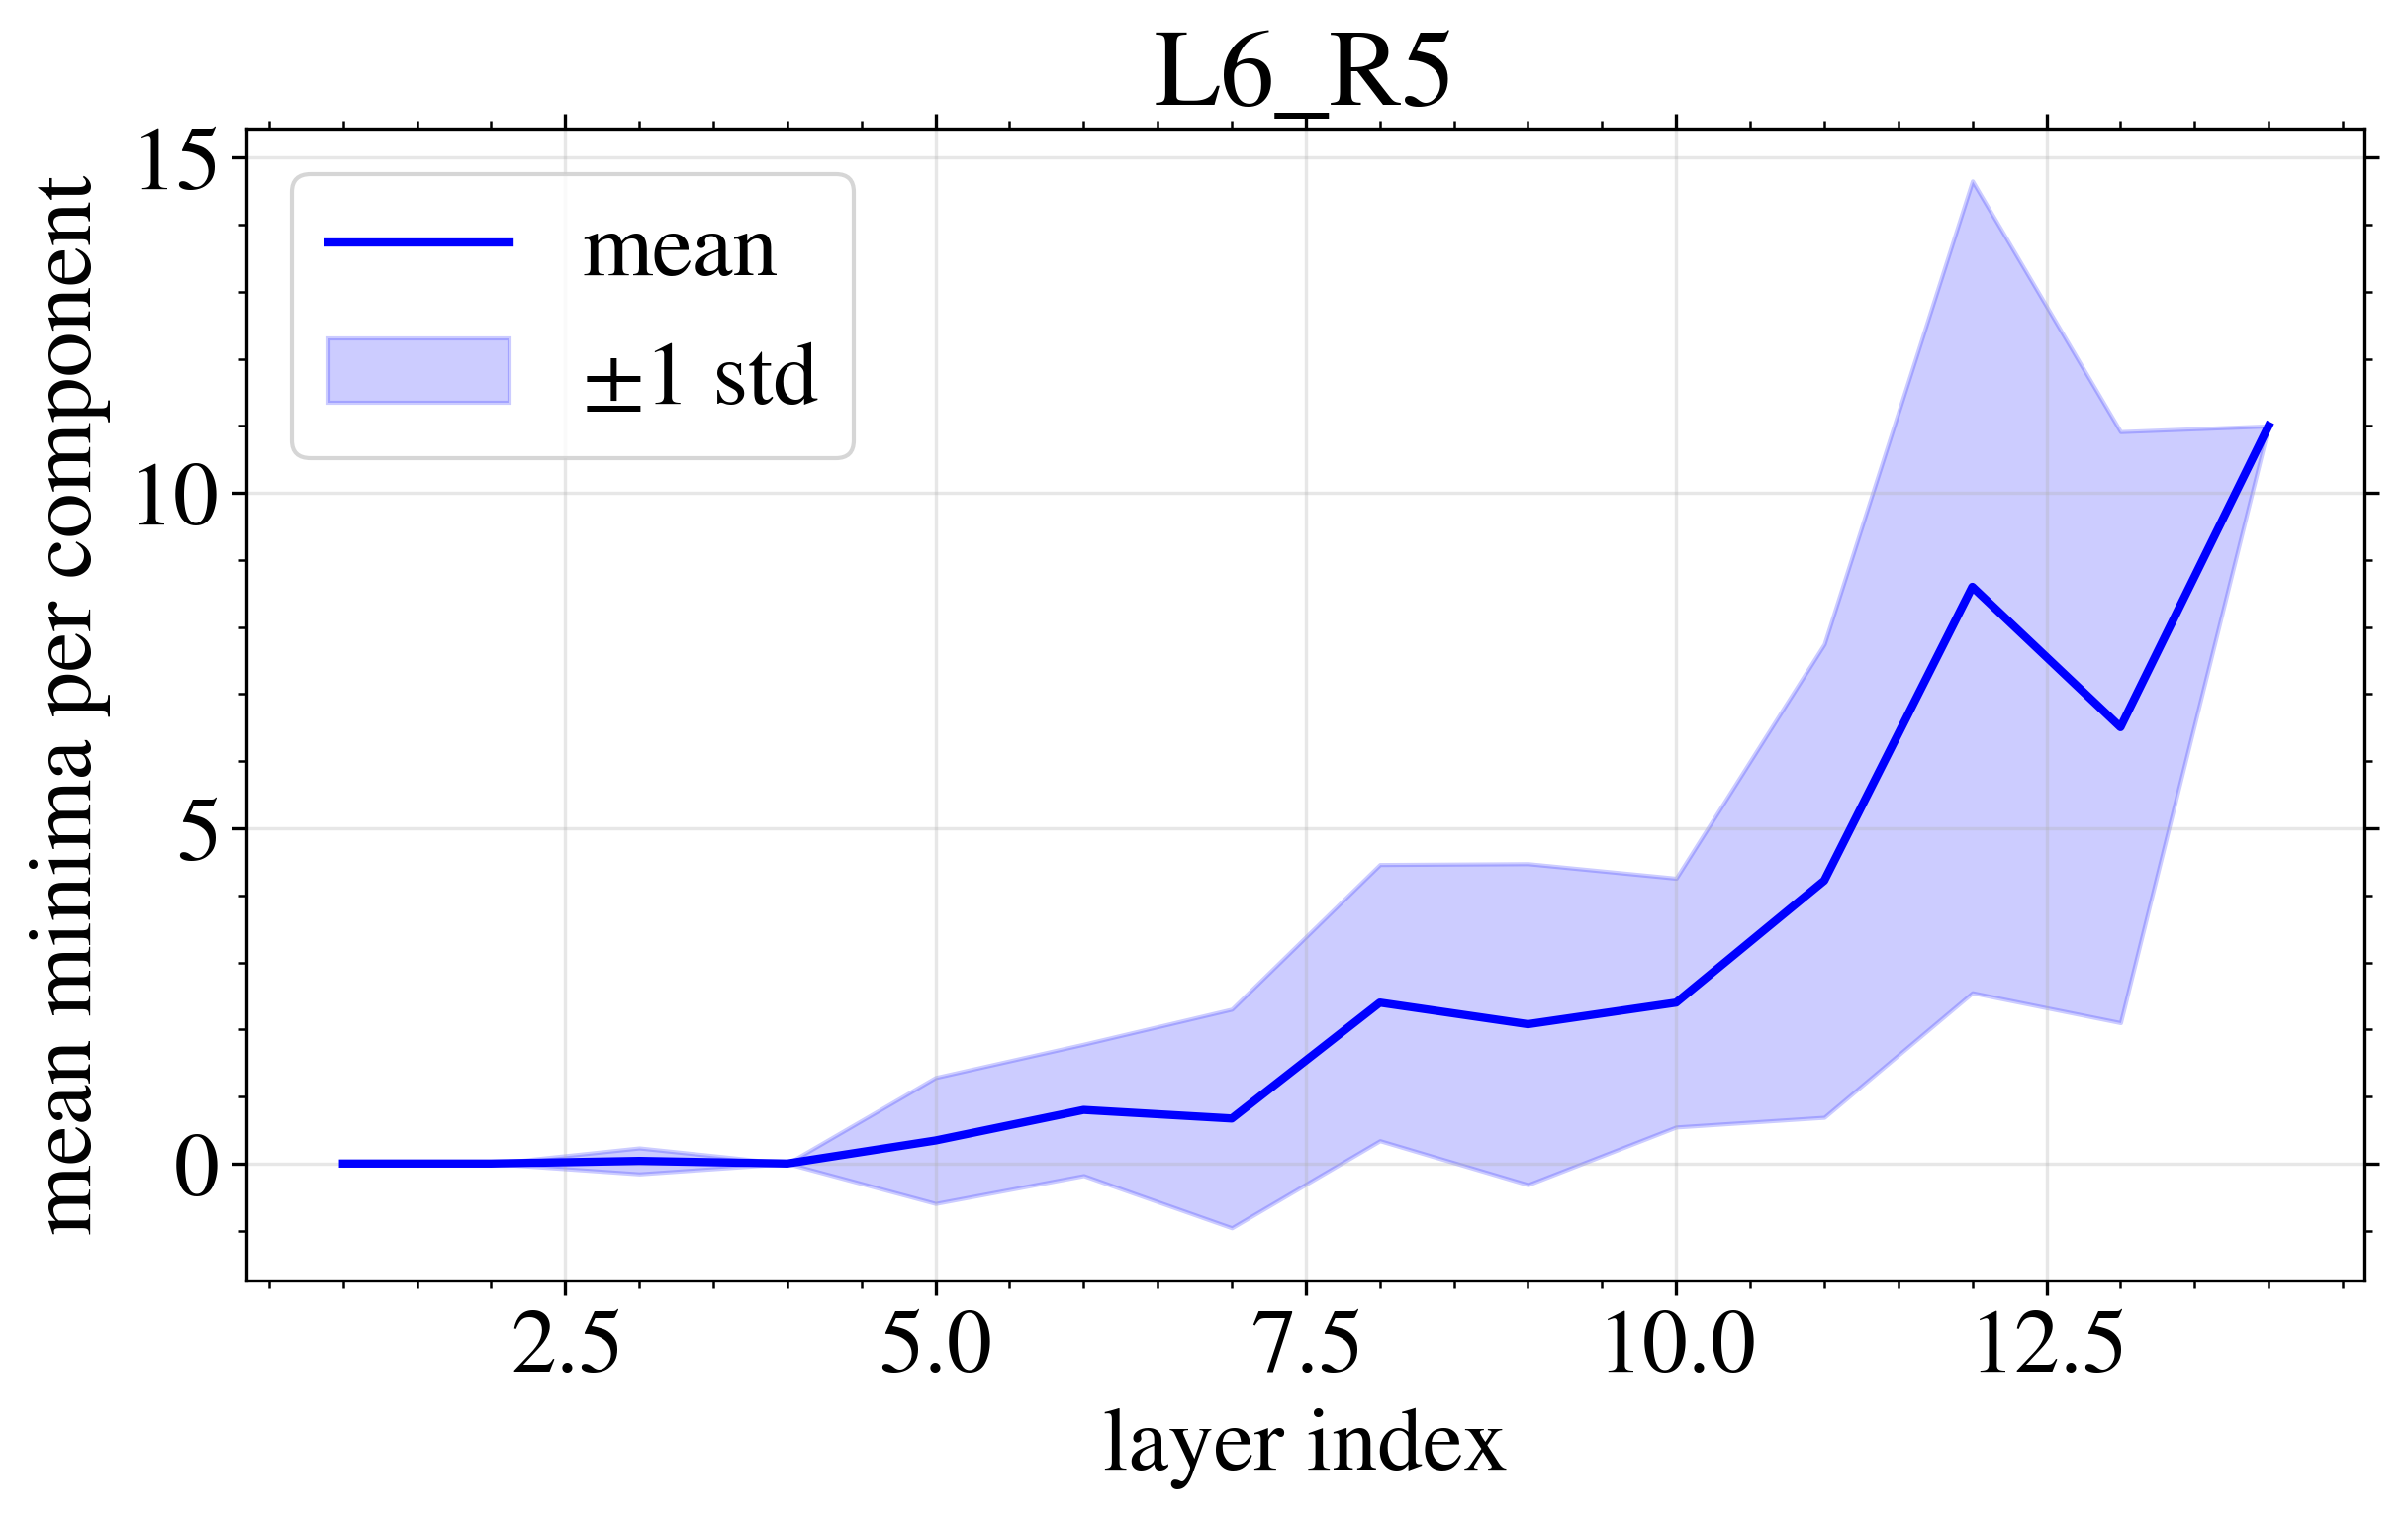
\includegraphics[width=0.85\linewidth]{../../experiments/partialfunctionanalysis/output_leap_all_L6_W128_grouped/grouped/L6_R5/mean_minima_per_component_vs_layer.png}
\caption{Mean number of strictly-positive local minima per component vs.\ layer index $\ell$, for MMNN with $L=6$, $W=128$, $R=5$. Error bands show $\pm$1 standard deviation across components.}
\label{fig:mean-minima-vs-layer}
\end{figure}

\subsection{Limitations and follow-ups}

Limitations: (1) no seed replication---each $(L,W,R)$ currently has one run; (2) grid resolution---the minima count is a lower bound, so faster oscillations may be under-counted; (3) the last layer is scalar in our setup; (4) conclusions are restricted to the specific 1D regression task and the $L,W,R$ range used. Suggested follow-ups: multiple seeds per config with error bars; optionally a Fourier-based metric (e.g.\ spectral centroid); extension to other depths and widths.

\section{Discussion}

The log-ratio $R_{ij}(t,x)$ is a simple diagnostic for channel-wise feature learning; the conditional theorem and two-sided step toy model specify when dominance is maintained. Mean-field two-step and cosine experiments (channel shares at spike locations, log-ratios over time) show increasing channel specialization in agreement with this picture. The oscillatory-complexity study provides empirical evidence that deeper layers exhibit higher mean minima per component (e.g.\ $\bar{m}_\ell \le 0.35$ in layers 1--4 vs.\ 2--9 in late layers at $L=6$, $W=128$), consistent with depth supporting higher-frequency structure; rank $R$ modulates the curves without a monotonic trend in the current data. Both strands align with the SciForDL goal of controlled experiments to formulate and test precise hypotheses about deep learning.

\bibliography{iclr2026_conference}
\bibliographystyle{iclr2026_conference}

\appendix
\section{Reproducibility}
The partial-function minima analysis can be reproduced with the repository script \texttt{positive\_local\_minima\_analysis.py} (see \texttt{experiments/partialfunctionanalysis/RESULTS\_ANALYSIS.md} for commands and outputs). Aggregated statistics (mean $\bar{m}_\ell$ per layer and per group, quantiles across components) are written to \texttt{group\_layer\_stats.csv} and \texttt{group\_summary.json} under \texttt{output\_leap\_all\_L6\_W128\_grouped/}; the figure used here is \texttt{grouped/L6\_R5/mean\_minima\_per\_component\_vs\_layer.png}.

\newpage
\section{Science of DL Improvement Challenge Submission}

\subsection{What model are you targeting?}
Low-rank neural networks (RF-LR and MMNNs) for 1D regression and scientific-computing-style targets (hierarchical Fourier, sum of cosines). We target understanding of their feature learning (channel specialization, log-ratio dynamics) and oscillatory complexity across layers.

\subsection{How do your results contribute—or could potentially contribute—to understanding these models?}
We provide a conditional theorem and toy model for when channel dominance is maintained (log-ratio criterion) and an empirical proxy (mean minima per component) showing that deeper layers learn more oscillatory partial functions, with a reproducible pipeline to refine or falsify the claim.

\subsection{How do you expect your submission to influence future work?}
The log-ratio diagnostic and the minima-count statistic can be adopted in other architectures and tasks; the oscillatory-complexity protocol can be extended with multiple seeds and Fourier-based metrics to strengthen scaling claims about depth and rank.

\end{document}
